En este capítulo se presentará el estado del arte en lo que respecta a los distintos usos de las bioseñales. Se brindarán algunos ejemplos del uso de las bioseñales en distintos campos.

\section{\acrshort{acat}}

La computadora utilizada por Stephen Hawking es tal vez el caso más conocido de la utilización de bioseñales en Accesibilidad. Stephen Hawking cuenta con esclerosis lateral amiotrófica, por lo que se encuentra paralizado y no puede hablar. Para poder comunicarse, Intel desarrolló un sistema compuesto por una tableta y un sensor infrarojo montado sobre sus anteojos. El sensor infrarojo detecta el movimiento en su mejilla izquierda. La tableta cuenta con una plataforma de código abierto llamada \acrshort{acat}. \acrshort{acat} provee un teclado virtual en la pantalla. Utilizando el movimiento de su mejilla, Hawking, puede detener el cursor donde desea y así, escribir. Es decir, es una entrada binaria. Este también utiliza un procesador de texto con predicción de palabras que permite acelerar el proceso.  Luego, el sistema utiliza un sintetizador de voz para comunicar lo que escribió. Esta, es solo una de las aplicaciones de \acrshort{acat}. \acrshort{acat} también le permite controlar el ratón en \emph{Windows}, y así, controlar completamente la computadora para poder utilizar su correo electrónico, navegar por internet, entre otras cosas. \acrshort{acat} puede utilizar como entrada cualquier bioseñal. \cite{hawking}.

\section{Gestos Como Dispositivos de Entrada}

La \acrshort{nasa} desarrolló un sistema para controlar un avión en una simulación utilizando los movimientos musculares medidos con sensores EMG(Electromiografía). Colocaron diversos sensores sobre una manga de tela. Con ellos, adquirieron la señal y la filtraron y eliminaron el ruido. Luego extrajeron las características y reconocieron patrones en una fase de entrenamiento. Con esta información, se aplicaron patrones de reconocimiento en una simulación interactiva. Lograron controlar un avión de guerra sin utilizar una palanca de mando. Es decir, el usuario colocaba la mano como si estuviese utilizando una palanca de mando y realizaba movimientos para controlar el avión (ver figura \ref{fig:emg-flight}) \cite{emg-flight}.

\begin{figure}[H]
	\centering
    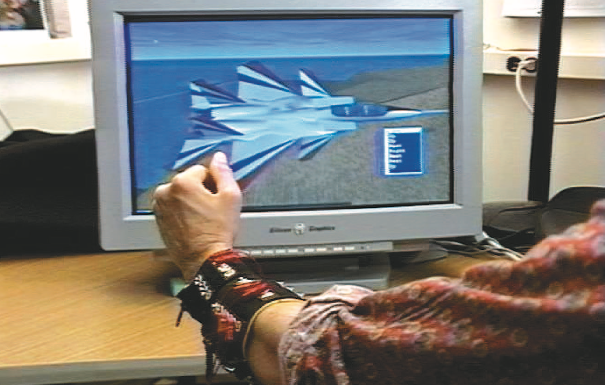
\includegraphics[width=0.8\textwidth]{emg-flight.png}
    \caption{Un usuario utilizando el dispotivo EMG para controlar un avión en una simulación  \cite{emg-flight}.}
	\label{fig:emg-flight}
\end{figure}

\section{\emph{Muscleman}}

Dos académicos de la Universidad Nacional de Seúl, utilizaron un dispositivo \acrshort{emg} y un acelerómetro para controlar un vídeojuego. Utilizando el acelerómetro, el juego era capaz de determinar si el usuario estaba dando un simple puñetazo hacia adelante, un puñetazo de abajo hacia arriba o si estaba lanzando una bola de fuego (ver figura \ref{fig:fireball}). Usando el sensor EMG, el juego medía la fuerza realizada por el usuario y la aplicaba proporcionalmente en el juego. Es decir, si el usuario realizaba poca fuerza, el ataque era débil. En cambio, si era fuerte, el ataque era fuerte. De esta forma, se utilizó como dispositivo de entrada las propias señales del cuerpo en lugar de usar un control de mando físico o el teclado \cite{emg-fireball}.

\begin{figure}[H]
    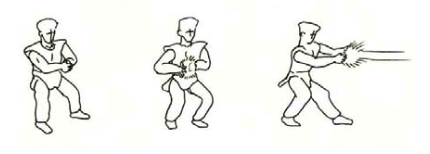
\includegraphics[width=0.8\textwidth]{emg-fireball.png}
    \caption{Movimiento que debe realiza un usuario para lanzar una bola de fuego en el videojuego \emph{Muscleman} \cite{emg-fireball}.}
	\label{fig:fireball}
\end{figure}

\section{\emph{Muse}}

La empresa \emph{Muse} desarrolló un dispositivo \acrshort{eeg} con siete electrodos. El mismo viene acompañado con una aplicación móvil que ayuda a los usuarios a meditar. Cuando el usuario tiene la mente tranquila, se escucha un clima calmo, pero cuando el usuario está alterado se escucha un clima tormentoso. Muse utiliza distintas ondas cerebrales para detectar si el usuario se encuentra relajado o no.

\section{\emph{MindFlix}}

\emph{Netflix} desarrolló \emph{MindFlix}. \emph{Mindflix} utiliza un dispositivo \acrshort{eeg} para controlar su popular servicio con la mente. Utiliza el giroscopio y el acelrómetro del dispositivo para permitirle al usuario desplazarse horizontalmente y verticalmente por la interfaz. Además, utiliza distintas ondas cerebrales para detectar cuando el usuario piensa en la palabra \emph{play}. En caso de que el usuario piense en esa palabra,  la aplicación comienza a reproducir el contenido seleccionado. Se intentó averiguar qué ondas cerebrales se utilizaban y de que forma, pero no se encontró en ningún lugar \cite{mindflix}.


\section{\emph{Neurogaming}}

\emph{Neurogaming} es la utilización de \acrshort{bci} en videojuegos para mejorar la experiencia. El concepto surgió hace algunos años pero aún no se ha explorado mucho. Existe muy pocas aplicaciones comerciales de este tipo. Un ejemplo es \emph{Throw Trucks With Your Mind} el cuál utiliza las ondas \emph{Beta} del cerebro para lanzar camiones \cite{neurogaming}.


